\documentclass[12pt]{article}
\setlength{\oddsidemargin}{0in}
\setlength{\evensidemargin}{0in}
\setlength{\textwidth}{6.5in}
\setlength{\parindent}{0in}
\setlength{\parskip}{\baselineskip}
\usepackage{amsmath,amsfonts,amssymb}
\usepackage{graphicx}
\usepackage{enumitem}
\usepackage[]{algorithmicx}
\usepackage{amsthm}
\usepackage{fancyhdr}
\pagestyle{fancy}
\setlength{\headsep}{36pt}
\usepackage{tkz-berge}
\usetikzlibrary{positioning, automata}

\usepackage{hyperref}

\theoremstyle{remark}
\newtheorem*{solution}{Solution}

\newcommand{\makenonemptybox}[2]{%
%\par\nobreak\vspace{\ht\strutbox}\noindent
\item[]
\fbox{% added -2\fboxrule to specified width to avoid overfull hboxes
% and removed the -2\fboxsep from height specification (image not updated)
% because in MWE 2cm is should be height of contents excluding sep and frame
\parbox[c][#1][t]{\dimexpr\linewidth-2\fboxsep-2\fboxrule}{
  \hrule width \hsize height 0pt
  #2
 }%
}%
\par\vspace{\ht\strutbox}
}
\makeatother

\begin{document}
\definecolor {processblue}{cmyk}{0.96,0,0,0}

\lhead{{\bf CSCI 3104, Algorithms \\ Problem Set 5b (48 points)} }
\rhead{Name: Luna McBride \\ ID: 107607144 \\ {\bf Profs.\ Hoenigman \& Agrawal\\ Fall 2019, CU-Boulder}}
\renewcommand{\headrulewidth}{0.5pt}

\phantom{Test}

\begin{small}
\textbf{Instructions for submitting your solution}:
\vspace{-5mm} 

\begin{itemize}
	\item The solutions \textbf{should be typed} and we cannot accept hand-written solutions. \href{http://ece.uprm.edu/~caceros/latex/introduction.pdf}{Here's a short intro to Latex.}
	\item You should submit your work through \href{https://www.gradescope.com/courses/59294}{\textbf{Gradescope}} only.
	\item If you don't have an account on it, sign up for one using your CU email. You should have gotten an email to sign up. If your name based CU email doesn't work, try the identikey@colorado.edu version. 
	\item Gradescope will only accept \textbf{.pdf} files (except for code files that should be submitted separately on Gradescope if a problem set has them) and \textbf{try to fit your work in the box provided}. 
	\item You cannot submit a pdf which has less pages than what we provided you as Gradescope won't allow it. 
	\item Verbal reasoning is typically insufficient for full credit. Instead, write a logical argument, in the style of a mathematical proof.
	\item For every problem in this class, you must justify your answer:\ show how you arrived at it and why it is correct. If there are assumptions you need to make along the way, state those clearly.
	
	\item You may work with other students. However, \textbf{all solutions must be written independently and in your own words.} Referencing solutions of any sort is strictly prohibited. You must explicitly cite any sources, as well as any collaborators. 
\end{itemize}



\vspace{-4mm} 
\end{small}

\hrulefill

\newpage
\begin{enumerate}

\item (25 pts) For this question, you are going to implement Kruskal's algorithm and union-find to build an MST from supplied data. Refer to the python starter code \textbf{MST\_Q1\_starter\_code.py} on Canvas that generates a graph of US cities, where the cities are the vertices and the edges are the distances between them. The code requires \textbf{miles\_dat.txt.gz} file as the graph data source so keep it in the same folder as the code. Before you start writing any code, make sure you can build the code that's been supplied. The code uses the networkx library. You may need to install this library for the code to run.

\textbf{Read all instructions for this question carefully.} 

\begin{enumerate}[label=(\alph*)]

\item (5 pts) Complete the code to find the edges that are part of the MST. You should add these edges in the list $kruskal\_selected\_edges$. Do not change the existing format of the edges. They are represented as a tuple of vertices and a vertex is represented like $v = \text{"Waukegan, IL"}$. Read the comments in the code for more information. You don't need to read/understand the $miles\_graph()$ and $draw\_graph()$ functions. 

\item (10 pts) Implement the $union()$ function to implement Kruskal's.\\


\item (10 pts) Modify your code slightly so that you can produce disconnected components. Let's call these components clusters. The “spacing” of any particular clustering (group of clusters) is defined as the smallest edge between vertices in any pair of different clusters. If we stop Kruskal's $k$ iterations before the algorithm completes, what is the spacing value? Run your code for $k = 2...10$ to generate spacing for all these k values. Your code needs to have this calculation for your answer to receive credit. \\
\item In the pdf that you submit for this assignment, please include the following:
\begin{enumerate}
    \item One of the generated graphs \textbf{MST.png} that your code produces that shows the MST for that run. Note that on each run, you can get a different number of edges to begin with. Thus, you can expect a different answer each time you run.
    \item The spacing values for each $k$ value that you use.
    \item Your .py file for this question needs to be submitted to Canvas.
\end{enumerate}
\pagebreak

(Space for Q1 image and spacing values)
\begin{solution}
$\newline$ Spacing value for each k: $\newline$ 
[('Santa Barbara, CA', 'Salinas, CA') ('Sterling, CO', 'Salida, CO'), ('Valley City, ND', 'Winnipeg, MB'), ('Roswell, NM', 'San Angelo, TX'), ('Salem, OR', 'Weed, CA'), ('Sheridan, WY', 'Scottsbluff, NE'), ('Williston, ND', 'Valley City, ND'), ('Scottsbluff, NE', 'Rock Springs, WY'), ('Twin Falls, ID', 'Walla Walla, WA'), ('San Diego, CA', 'Tucson, AZ')] $\newline$ $\newline$$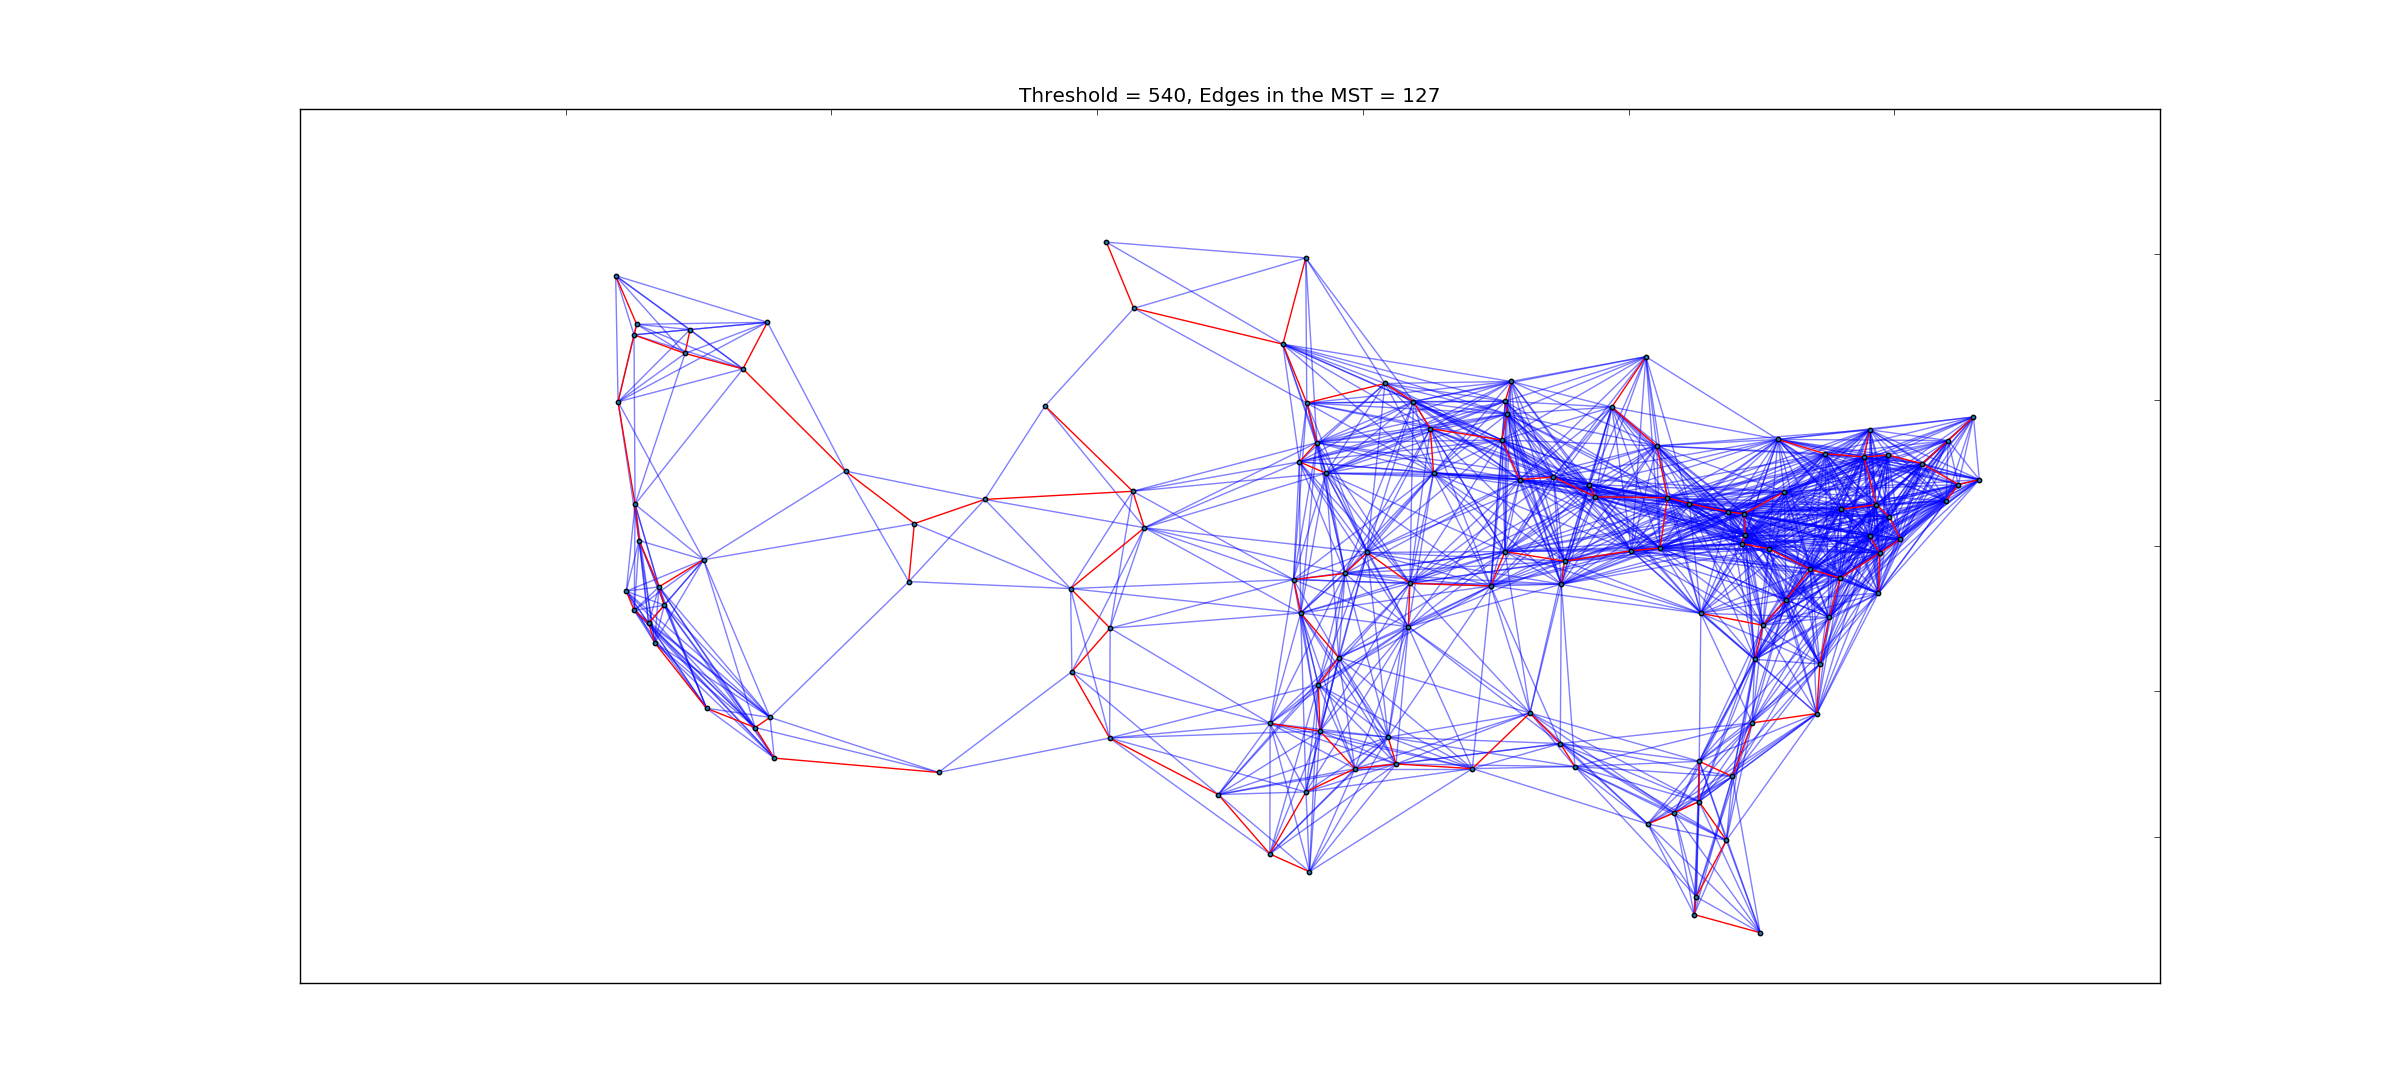
\includegraphics[width=6in,height=4.5in]{MSTGraph}$ 

\end{solution}

\pagebreak

\end{enumerate}

\item (3 pts) How many disconnected components are there when you stop Kruskal's $k$ round before you complete the MST? Justify your answer. 
\begin{solution}
$\newline$ For k iterations before Kruskal's stops, there are k+1 discomponents left. Since union connects 2 disconnected graphs, each iteration takes one graph out of the equation. That means for every run of the algorithm, one disconnected component is removed. We are looking for one connected whole at k=0 (the end of kruskals), and since the union brings 2 into 1, the step before must have 2 graphs. k=0$->$components=1, k=1$->$components=2. Therefore, k=k$->$components=k+1
\end{solution}


\item (5 pts) Consider the recurrence $F_{n} = 2F_{n-1} + F_{n-2}$, with the base cases $F_{0} = 1$ and $F_{1} = 2$. Suppose we have letters $v_{0}, \ldots, v_{7}$; where for $i \in \{0, \ldots, 7\}$, the frequency of $v_{i}$ is given by $F_{i}$. Draw a Huffman tree for $v_{0}, \ldots, v_{7}$. 

\begin{solution}
$\newline$$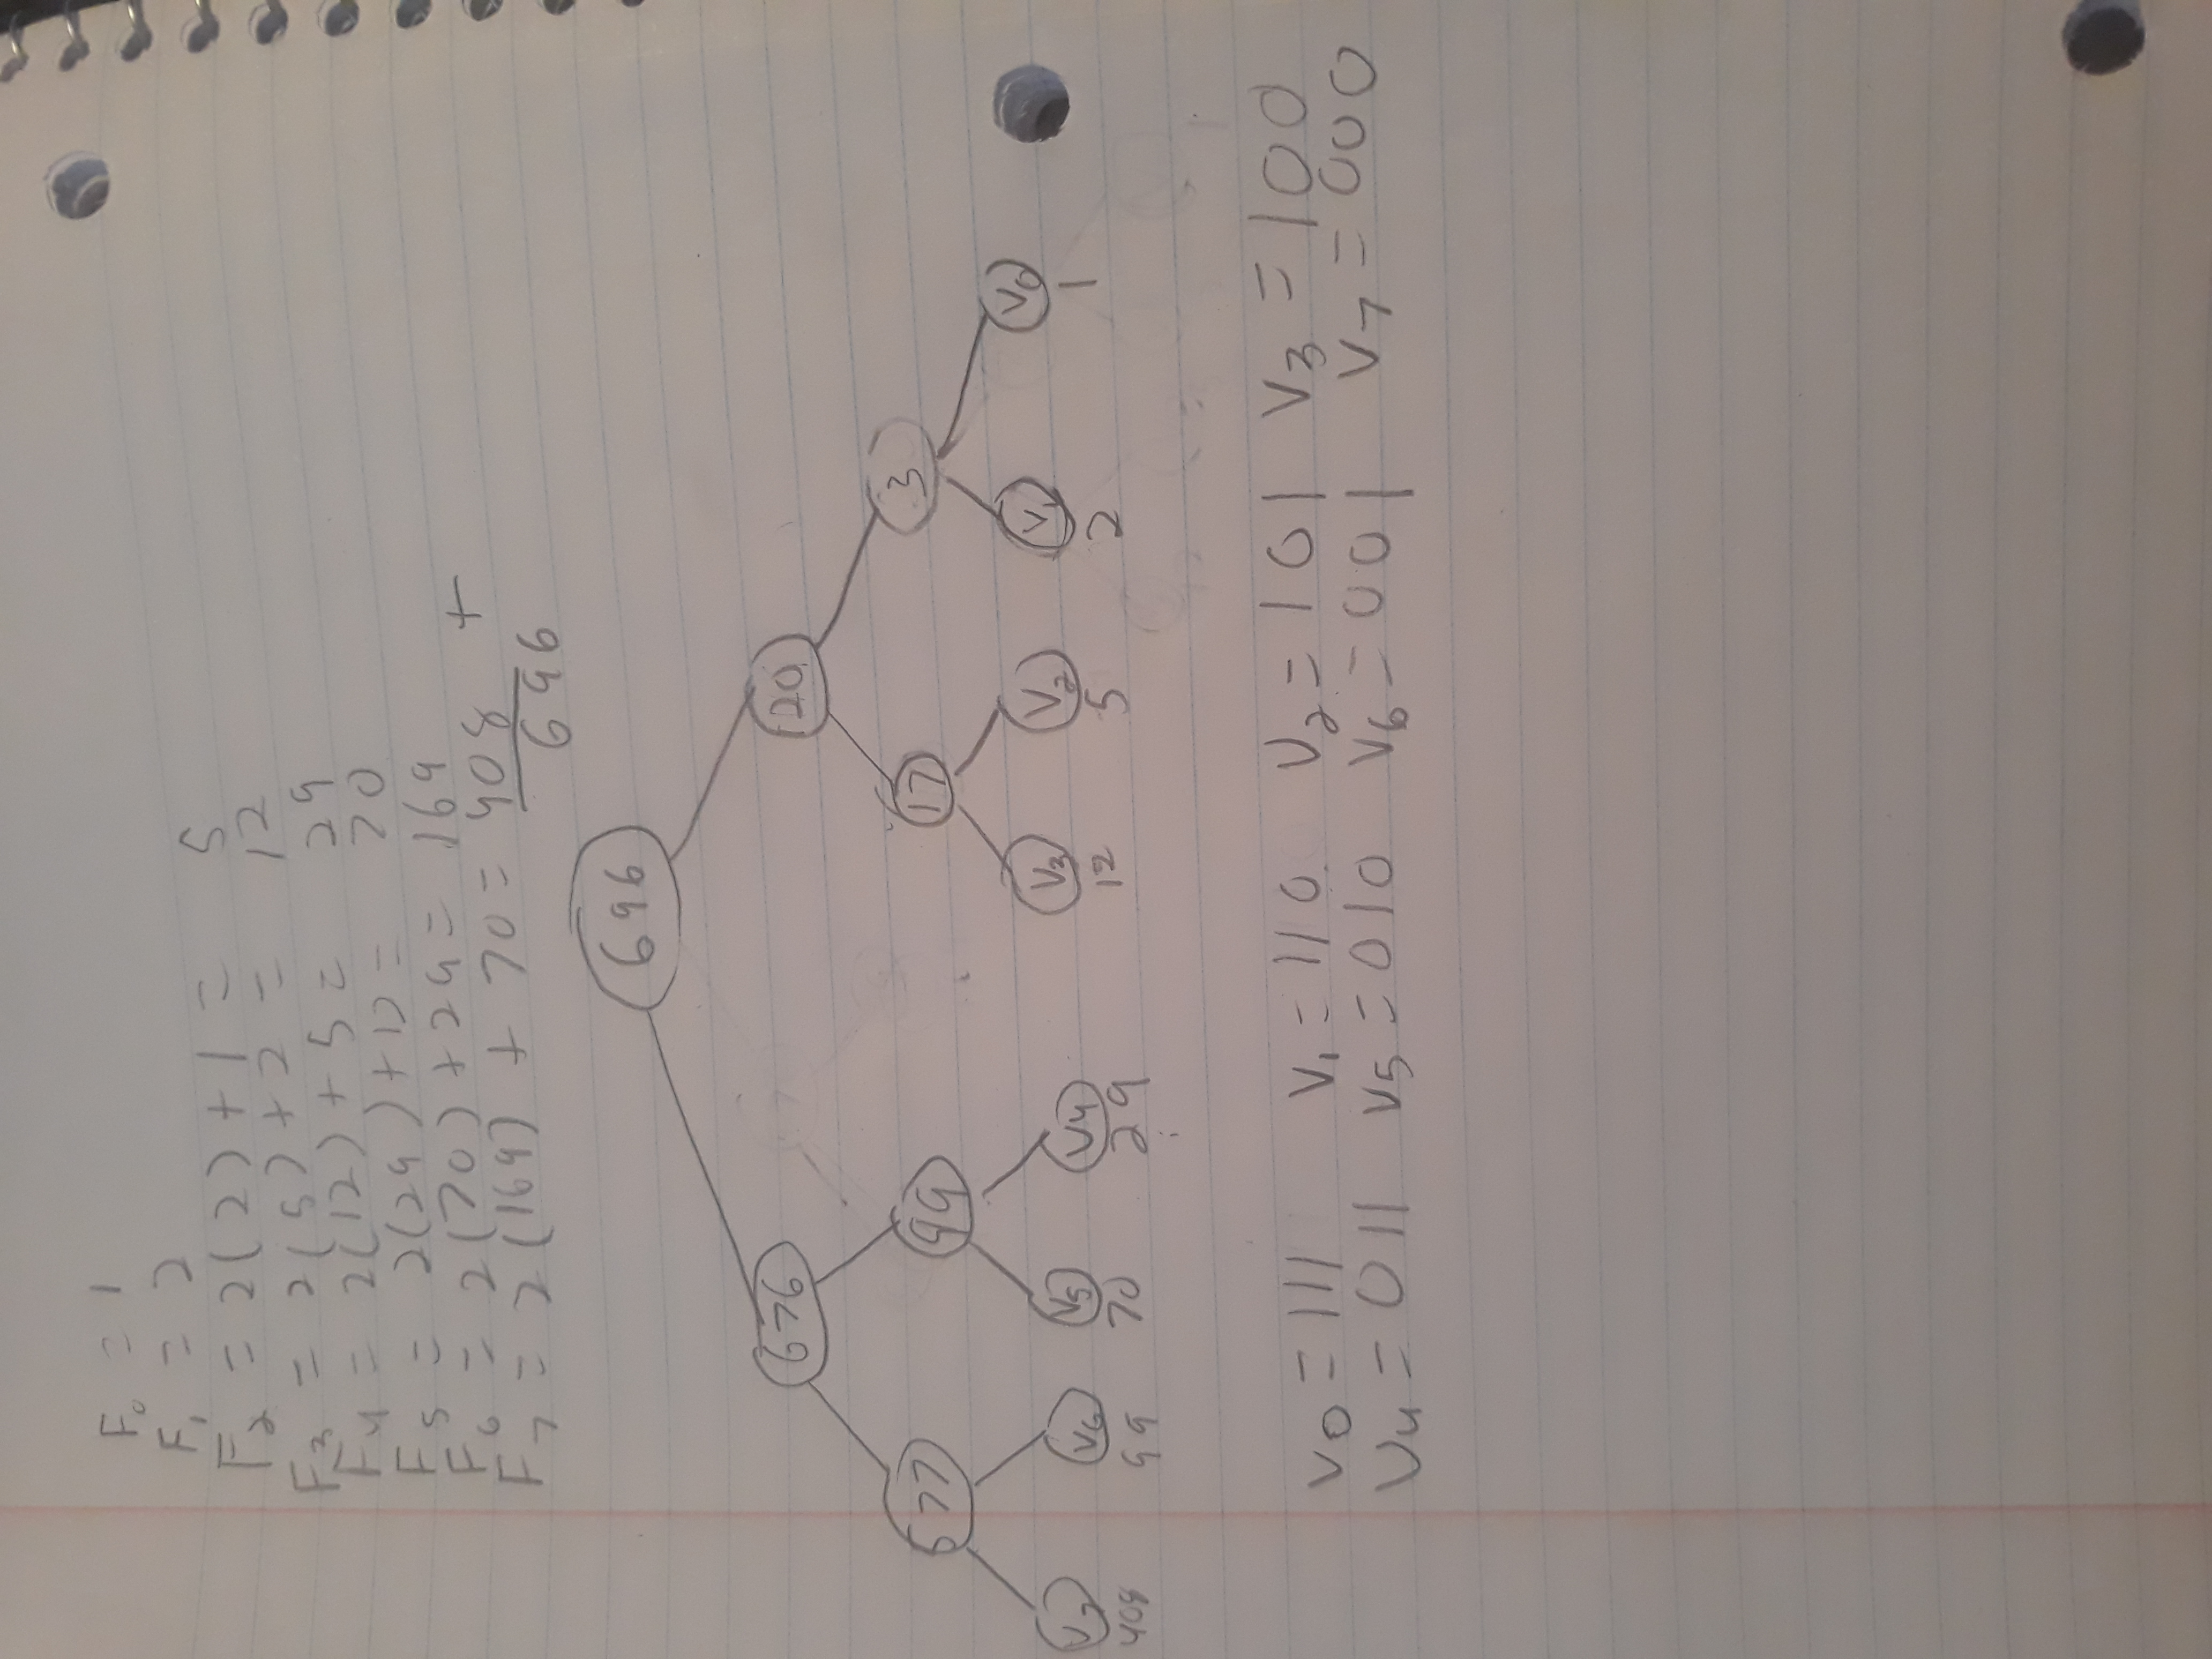
\includegraphics[width=5in,height=5in, angle=-90]{Huffman}$ 
\end{solution}
\pagebreak


\item (5 pts) Assume you run your Huffman tree algorithm and you produce the following pre-fix codes. Describe why there must be an error in your algorithm.
\begin{verbatim}
    S = 00
    c = 01
    i = 001
    e = 011
    n = 101
\end{verbatim}
\begin{solution}
$\newline$ Let us take the value 001. This looks like it is 'i', but for all we know, it could be 'S' with the beginning part of 'n'. Imagine this in a very long string where these sort of issues persist. $\newline$ Since Huffman trees are meant to prevent this ambiguity, there had to have been an error in the algorithm
\end{solution}
\pagebreak

\item (10 pts) Assume you're given an integer matrix that represents a plot of land, where the value at that location in the matrix represents the height above sea level. A value of zero indicates water. A pond is a region of water connected vertically, horizontally, or diagonally. The size of the pond is the total number of connected water cells. Write an algorithm to compute the sizes of all ponds in the matrix.

Example:
\begin{verbatim}
    0 2 1 0
    0 1 0 1
    1 1 0 1
    0 1 0 1
\end{verbatim}

would output 1, 2, 4.
\begin{enumerate}
    \item (3 pts) Describe the graph data structure that your algorithm will use for this problem.
    
    \begin{solution}
	$\newline$ For this, I will only be counting the 0's in our graph. This is an unweighted, undirected graph connecting adjacent 0's. Each pond would be a disconnected component in terms of the graph, just as the map works in question 1 (The area not considered on the US map exists, but it is not considered in that circumstance), for example.
    \end{solution}
\pagebreak
    
    \item (2 pts) Provide a 3-4 sentence description of how your algorithm works, including how the matrix is converted to the graph, how adjacent vertices are identified, and how the algorithm traverses the graph to identify connected vertices.
    
    \begin{solution}
	$\newline$The algorithm will take the array, read through it, and put every 0 as its own component. It will be holding the place in the array it exists in as well. The algorithm will then go through the list of 0's we have disconnected and look for those that are around it (for [1,1], the adjacent are all possibilities of adding or subtracting 1 from the 2d array, so [0,0],[0,1],[0,2],[1,0],[1,2],[2,0],[2,1],[2,2]). It will then go through to find the amount of ponds, then return them and their sizes via a list.
    \end{solution}
    
    \item (5 pts) Write an algorithm to solve this problem. 
    
    \begin{solution}
	$\newline$ pond(arr): $\newline -->$ for i in range(0,len(width of array)) $\newline --/-->$ for j in range(0,len(width of array)) $\newline --/--/-->$ if [i,j] is a 0 $\newline --/--/--/-->$ make it its own node, store the [i,j] value, store the 0 in a list of 0's $\newline$ $\newline$ $\newline -->$ while list of 0's is not empty $\newline --/-->$ check adjacent array values for 0 $\newline --/-->$ if there is a 0 $\newline --/--/-->$ connect the nodes, make new adjacencies for them as a group, reinsert group to be checked for surrounding 0's $\newline$$\newline--/-->$ else $\newline --/--/-->$ remove the 0's from the 0's list, add the size of the group to the solution list $\newline$$\newline -->$ return solution list
    \end{solution}
    
\end{enumerate}


\end{enumerate}

\end{document}
